\chapter{The Unstructured Heart as a Binary Cube} 
After a MRI scan of the heart, the resulting data are stored as a point cloud, which is a huge collection of unstructured points, that typically needs advanced mesh generation techniques that consists of triangulations of the stored point cloud to form an accurate 3-D model of the human heart, that more specifically, is a large collection tetrahedras. 

The goal of my implementation is to generate a uniformly structured mesh, using the unstructured data as a basis for checking if a generated point is inside or outside the unstructured heart geometry. The resulting structured mesh will consist of points both inside and outside the heart, but will later be numerically masked away. A detailed description of the numerical strategy will be provided later in section X.X.

\section{Motivation}
%%explain motivation behind doing this.
As [HEART BOOK]

\section{The Processing of Unstructured data}
The unstructured data, consisting of a collection of vertex points, edges, faces, and a description of neighbouring elements comes in several different files. In the process of generating the structured mesh from the unstrctured data, an extraction of the tetrahedras vertex points are the only necessary information needed, due to the reason that you only need to check if a generated point is inside or outside a given tetrahedra. The complete process of mesh generation can be found later in section \ref{generating_the structured_mesh}.

For the process of extracting the vertex information of a tetrahedra, two files has to be read, an element (.ele) and a node (.node) file, both of which are of ASCII[FOOTNOTE] form.

\subsection{.node file}
\begin{lstlisting}[caption=.node file]
First line:	<# of points> <dimension (3)> <# of attributes>

Remaining lines list # of points:
				<point #> <x> <y> <z> 
				...
\end{lstlisting}
The .node file contains information of every vertex point of the unstructured mesh. The first line contains information of how many points there is, and in how many dimensions. The remaining lines contains a list of points. Each point, identified by an id, has a respective x, y and z coordinate, which reveals the position of the vertex point in the coordinate system.

%%KILDE: http://wias-berlin.de/software/tetgen/files/tetgen-manual.pdf

\subsection{.ele file}
\begin{lstlisting}[caption=.ele file]
First line:	<# of tetrahedra> <nodes per tet. 4>

Remaining lines list # of tetrahedra:
				<tetrahedron #> <node (point #)> <node (point #)> ... 
				...
\end{lstlisting}
The .ele files contains information relative to each respective tetrahedra. The first line contains information of how many tetrahedras there is, and how many nodes or vertex points there is per tetrahedra. The remaining lines contains an tetrahedra id and its respective vertex points. The unique node ids in the .ele file are used as indices into the corresponding .node file for extracting the vertex points. 
%%KILDE: http://wias-berlin.de/software/tetgen/files/tetgen-manual.pdf

Since there are no universal ordering of the tetrahedral mesh \cite{article4} the only viable option for storing the vertex points are in a 1D array. A complete random ordering of the vertex points results in cosequent random jumps in memory, resulting in poor computation speed \cite{article4}.

\begin{figure}[h]
 \centering 
     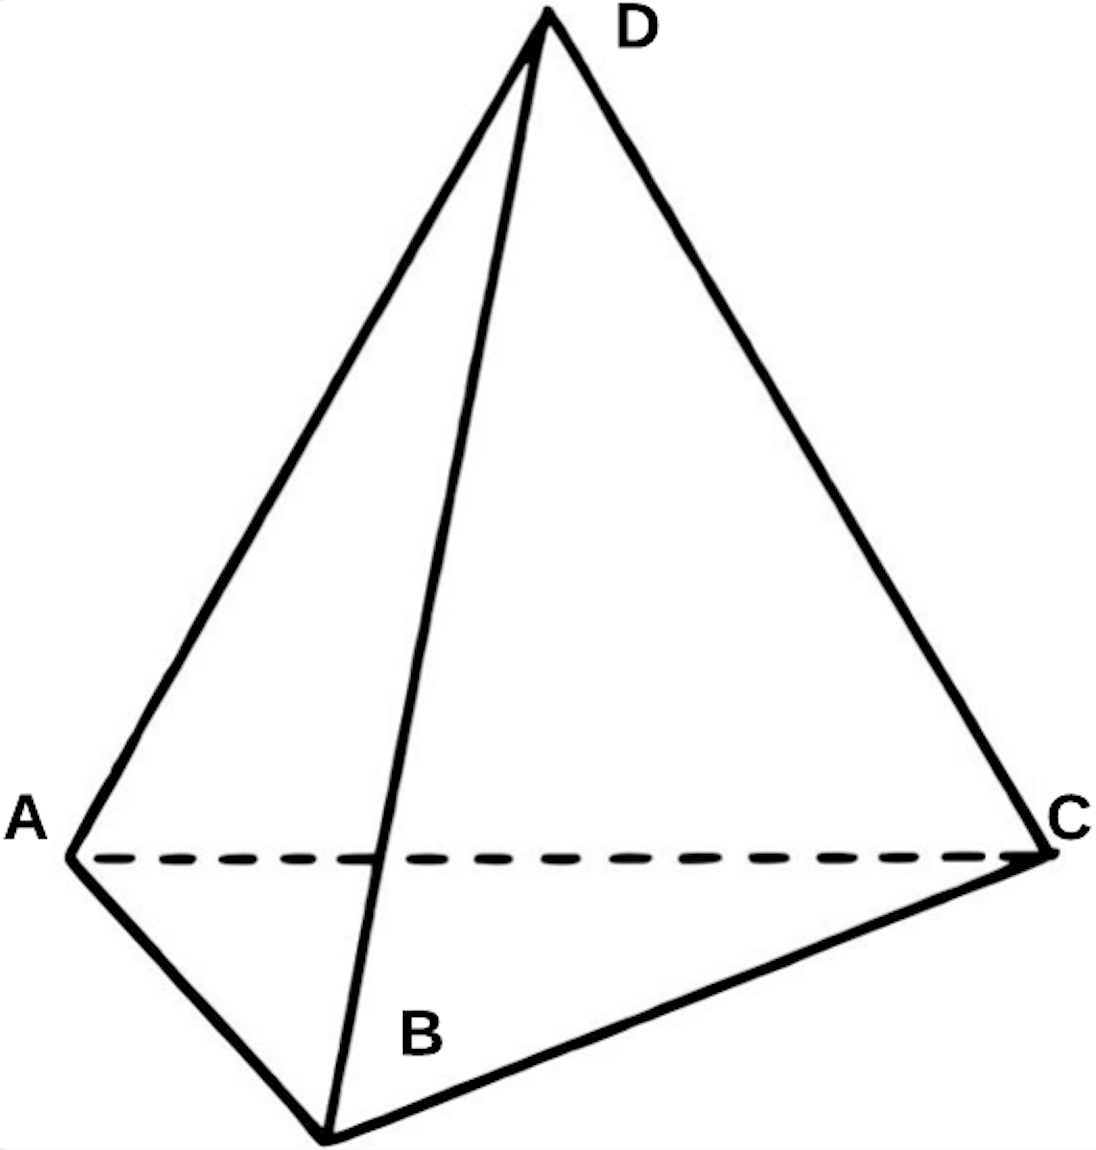
\includegraphics[scale=0.4]{bilder/m_tet}
     \caption{Illustration of a tetrahedra having 4 vertex points, A, B, C and D}.
     \label{m_tet.png}
\end{figure}


\section{Generating the Structured Mesh}
\label{generating_the structured_mesh}
Now that I have explained the pre processing steps of extracting the vertex points from the tetrahedral mesh, it is time to move on to the processing of the unstructured data, and the generation of the structured mesh.

For an ease of understanding the process of how the structured mesh is generated, most of the illustrations and examples will be coordinated in a 2D fashion.

\begin{figure}[h]
 \centering 
     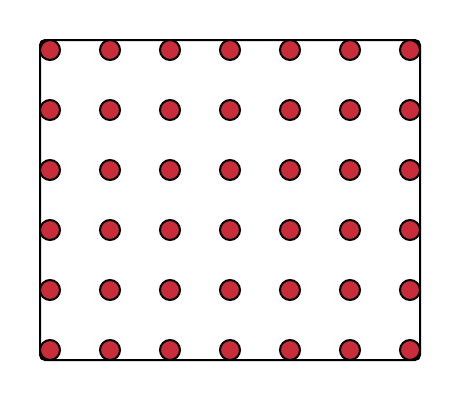
\includegraphics[width=0.9\textwidth]{bilder/m_grid_points}
     \caption{http://www.austincc.edu/rfofi/NursingRvw/PhysText/Cardiac.html}.
     \label{m_grid_points.png}
\end{figure}

Before filling the structured mesh with mesh points, I need to know the boundary values for the tetrahedral mesh, which involves computing the minimum and maximum values for the x, y and z coordinates in the coordinate system. The boundary values will be used as a upper and lower limit for the structured mesh, aswell as a stepping value for generating uniformly distributed mesh points. The stepping value is the distance between each mesh point in the structured mesh. The algorithm for determining the stepping value in the x, y and z direction is given in equation \ref{step}.
%%\begin{lstlisting}[caption={Cache Blocking} ,label={lst:stepx}]
%%step_x = (x_max - x_min)/nx;
%%\end{lstlisting}

\begin{equation} \label{step}
\textrm{Stepping value} = \frac{\textrm{Max value} - \textrm{Min value}}{\textrm{Number of points}} 
\end{equation}

Each respective mesh points can then be attained by following equation \ref{step} for calculating the x, y and z coordinate of each respective mesh point.

\begin{equation} \label{step}
\textrm{Mesh point} = \textrm{Min value} + (\textrm{stepping value} \times i)
\end{equation}

Where \(i\) is an increment of the total number of points in one direction. 


\begin{figure}[h]
 \centering 
     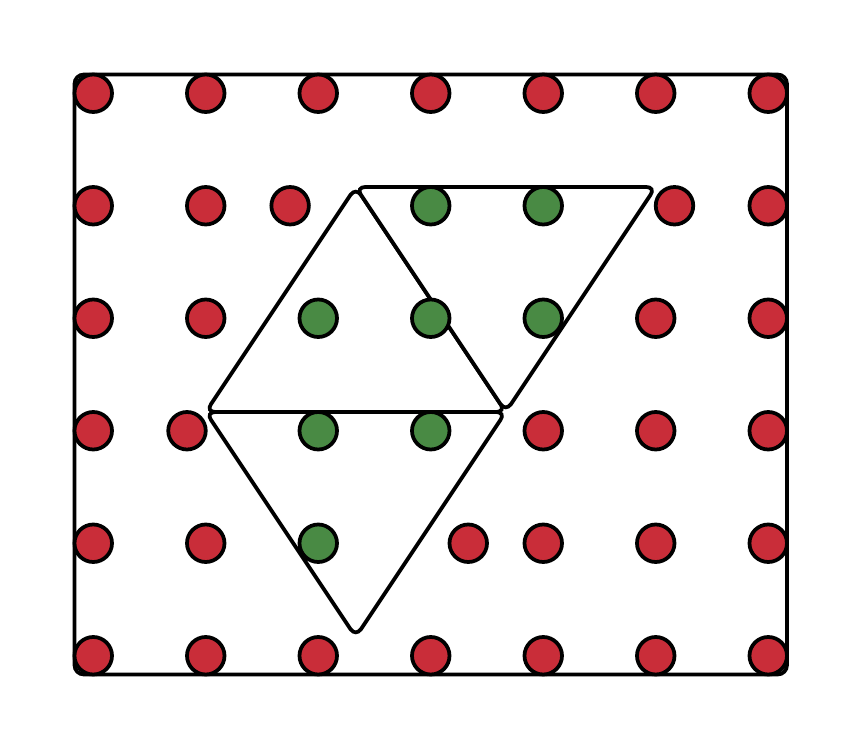
\includegraphics[width=0.9\textwidth]{bilder/m_points_inside}
     \caption{http://www.austincc.edu/rfofi/NursingRvw/PhysText/Cardiac.html}.
     \label{m_points_inside.png}
\end{figure}


\section{The Binary cube}
After the structured mesh has been filled with points, each point is checked with respect to the original 3D heart volume, being either inside or outside. More specifically, the mesh points is checked with respect to every tetrahedra in the unstructured mesh. The resulting data structured t is referred to as a binary cube, consisting of both the inside and outside points. The inside points will be given a numerical value which will be used later in the heart simulation, while the outside points are given a value to be identified commonly to all outside points.

The binary cube is a representation of all the generated points, stored in a 3D array. The process of filling the 3D binary cube with data yields a complexity of 4 for loops. The 3 outermost for loops iterates over the respective x, y, and z coordinates. While the innermost for loop iterates over every tetrahedron in the list, with the goal of extracting the x, y and z coordinates from the 4 vertices of every tetrahedron. The vertex points extracted from the tetrahedrons are used for the process of checking whether or not a generated point in the binary cube is inside the tetrahedron.

One approach of finding out if a point, \(P\) is inside a given tetrahedron, as given in [LINK], is to check if \(P\) and a tetrahedron vertex point \( V_{i}\) is on the same side of the boundary as \( i\). 
\[
V_{0} = (x_{0}, y_{0}, z_{0}) 
\]
\[
V_{1} = (x_{1}, y_{1}, z_{1})
\]
\[
V_{2} = (x_{2}, y_{2}, z_{2})
\]
\[
V_{3} = (x_{3}, y_{3}, z_{3})
\]

\[
P = (x, y, z)
\]
The first step of checking if a point is inside a tetrahedron involves computing the \(4 \times 4\) determinant of all the four vertices in the tetrahedron,  \(D_{0}\). The next step involves replacing one vertex point, with  \(P\), for all the vertices in the matrix. This results in a total of four, \(4 \times 4\) determinant operations, going from \(D_{1}\) to \(D_{4}\). 
\[
D_{0} =
\begin{vmatrix}
x_{0} & y_{0} & z_{0} & 1 \\ 
x_{1} & y_{1} & z_{1} & 1 \\ 
x_{2} & y_{2} & z_{2} & 1 \\ 
x_{3} & y_{3} & z_{3} & 1 \\ 
\end{vmatrix}
\]

\[
D_{1} =
\begin{vmatrix}
x & y & z & 1 \\ 
x_{1} & y_{1} & z_{1} & 1 \\ 
x_{2} & y_{2} & z_{2} & 1 \\ 
x_{3} & y_{3} & z_{3} & 1 \\ 
\end{vmatrix}
\]

\[
D_{2} =
\begin{vmatrix}
x_{0} & y_{0} & z_{0} & 1 \\ 
x & y & z & 1 \\ 
x_{2} & y_{2} & z_{2} & 1 \\ 
x_{3} & y_{3} & z_{3} & 1 \\ 
\end{vmatrix}
\]

\[
D_{3} =
\begin{vmatrix}
x_{0} & y_{0} & z_{0} & 1 \\ 
x_{1} & y_{1} & z_{1} & 1 \\ 
x & y & z & 1 \\ 
x_{3} & y_{3} & z_{3} & 1 \\ 
\end{vmatrix}
\]

\[
D_{4} =
\begin{vmatrix}
x_{0} & y_{0} & z_{0} & 1 \\ 
x_{1} & y_{1} & z_{1} & 1 \\ 
x_{2} & y_{2} & z_{2} & 1 \\ 
x & y & z & 1 \\ 
\end{vmatrix}
\]

The last and final step, involves comparing the signs of \(D_{i}\) to \(D_{0}\). If the sign of any \(D_{i}\) equals that of \(D_{0}\), then \(P\) is inside the boundary \(i\). If all the \(D_{i}\) share the same sign as \(D_{0}\), then the point \(P\) is inside all the 4 boundaries, and more specifically, \(P\) is inside the tetrahedron.


The experimental tests was conducted on an unstructured heart model consisting of 32
The generation of the binary cube is a time consuming process. Which at most, yields a total number of 
\begin{equation} 
X \times\ Y \times Z  \times \textrm{Total number of tetrahedrons}
\end{equation}  
iterations, and for an average case of 
\begin{equation} 
X \times\ Y \times Z  \times \frac{\textrm{Total number of tetrahedrons}}{2}
\end{equation} 
iterations.  

\section{The Simulation}
start of simulation

\section{Masking Away Outside Points}
Numerical strategy



%%Every point in the structured mesh has to be checked accordingly if


